
\renewcommand{\EntradaBibtex}{PinacotecaVirtual_2024}

\begin{frame}{\citetitle{\EntradaBibtex}$^*$ (1)}
\begin{block}{Motivación} 
Los recorridos virtuales ofrecen una herramienta valiosa para explorar y experimentar entornos tridimensionales, tanto en contextos educativos como recreativo.
\begin{itemize}
\item Se implementó una aplicación móvil para explorar de manera interactiva el museo virtual Pinacoteca de Tamaulipas. 
%\begin{itemize}
%\item Permite al usuario llevar el conteo de sentadillas, tanto se las hace de frente como de lado.
%\item Debe ubicar el dispositivo a una distancia de 80 cm. Si el ejercicio no es bien realizado, no se contabiliza.
%\end{itemize}
\end{itemize}
\end{block} 
%\begin{center}
%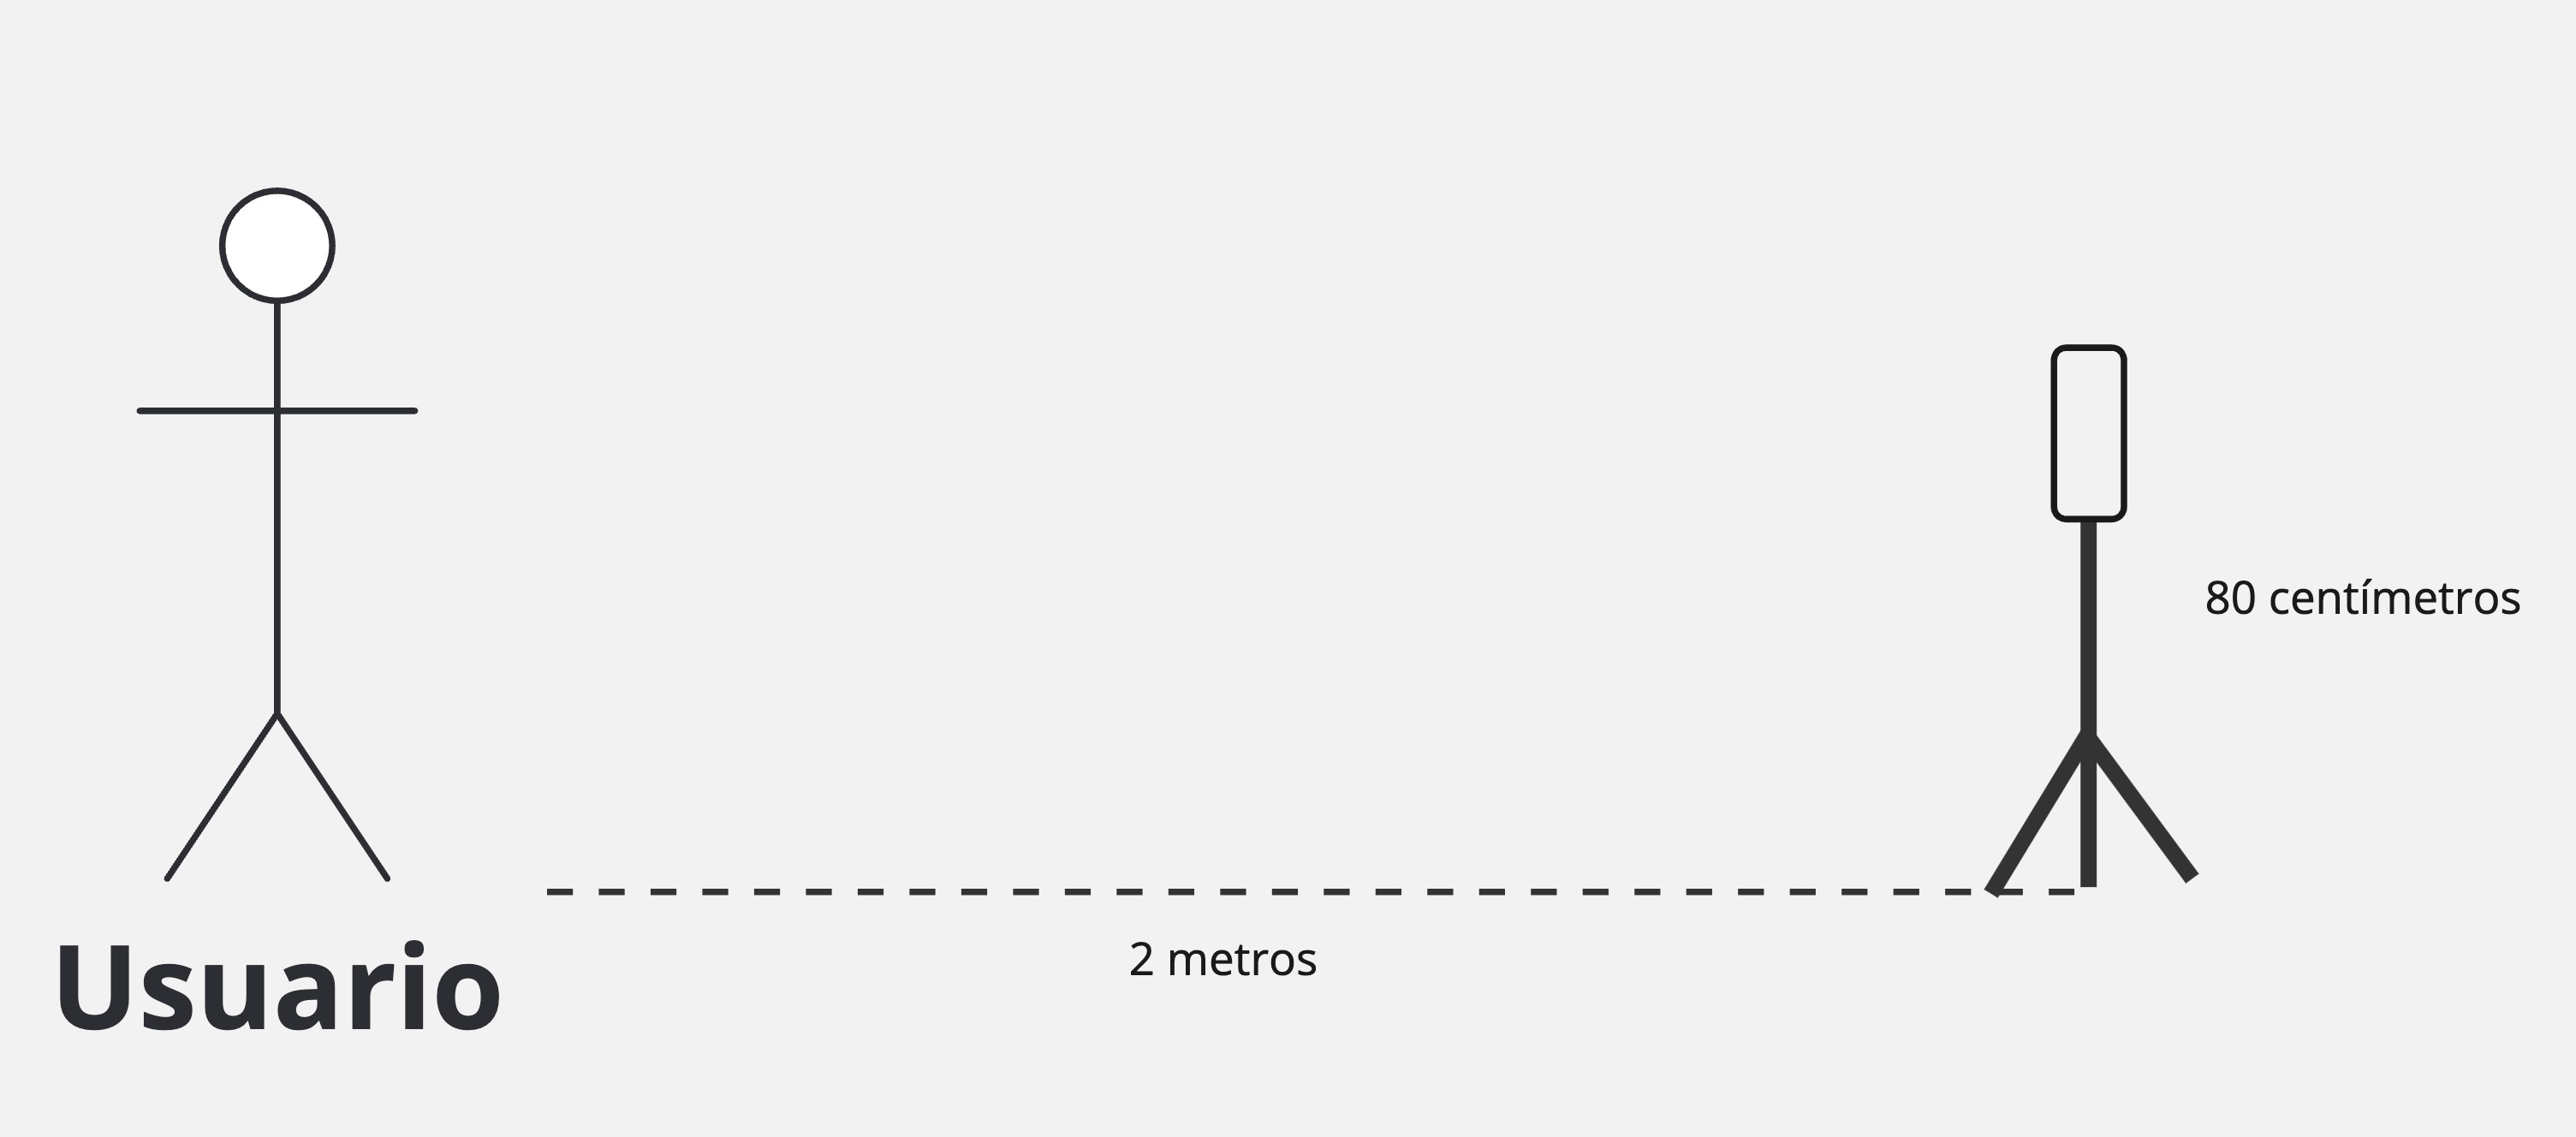
\includegraphics[width=0.48\linewidth]{2024_ConteoSentadillas/Ilustrativa.jpg}
%\end{center}
\footfullcite*{\EntradaBibtex}
\end{frame}


\begin{frame}{\citetitle{\EntradaBibtex} (2)}
%\begin{block}{Pantallas Principales} 

\begin{columns}
% Column 1
\column{.99\linewidth}



\begin{center}
	\begin{tabular}{cc}
		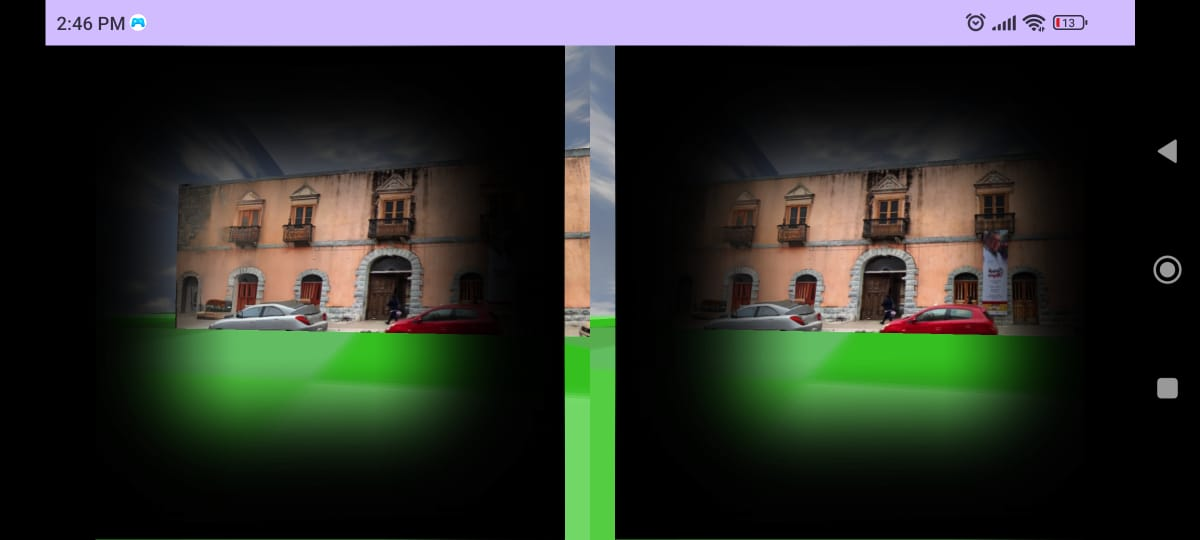
\includegraphics[width=0.40\linewidth]{2024_Pinacoteca_Virtual/EntradaPrincipal1.jpeg} &
		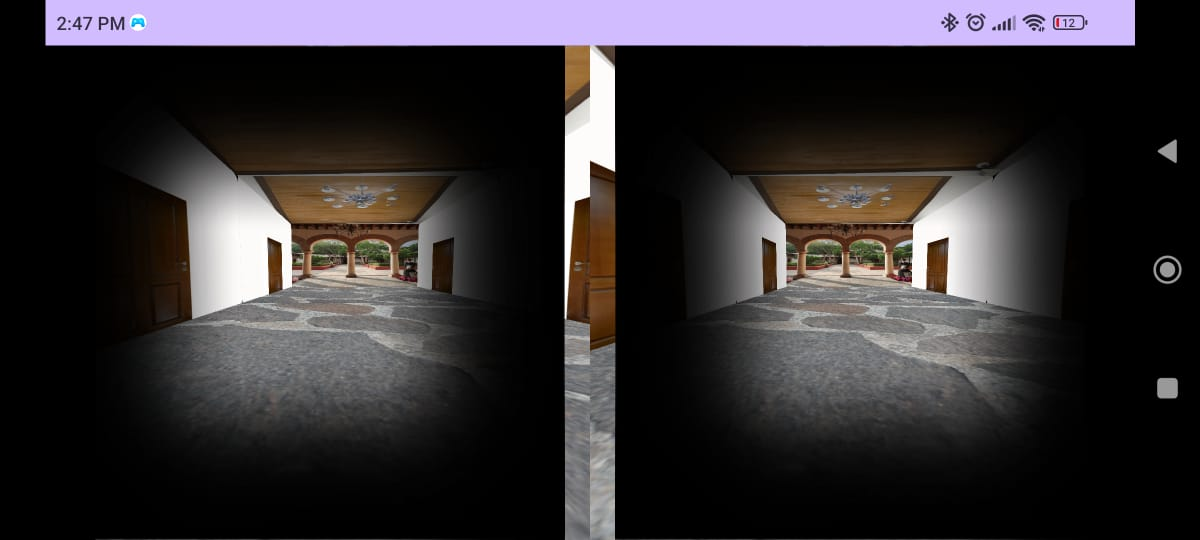
\includegraphics[width=0.40\linewidth]{2024_Pinacoteca_Virtual/EntradaPrincipal2.jpeg} \\
	\end{tabular}
\end{center}



%\column{.5\linewidth}
%\begin{center}
	%\begin{tabular}{cccc}
	%	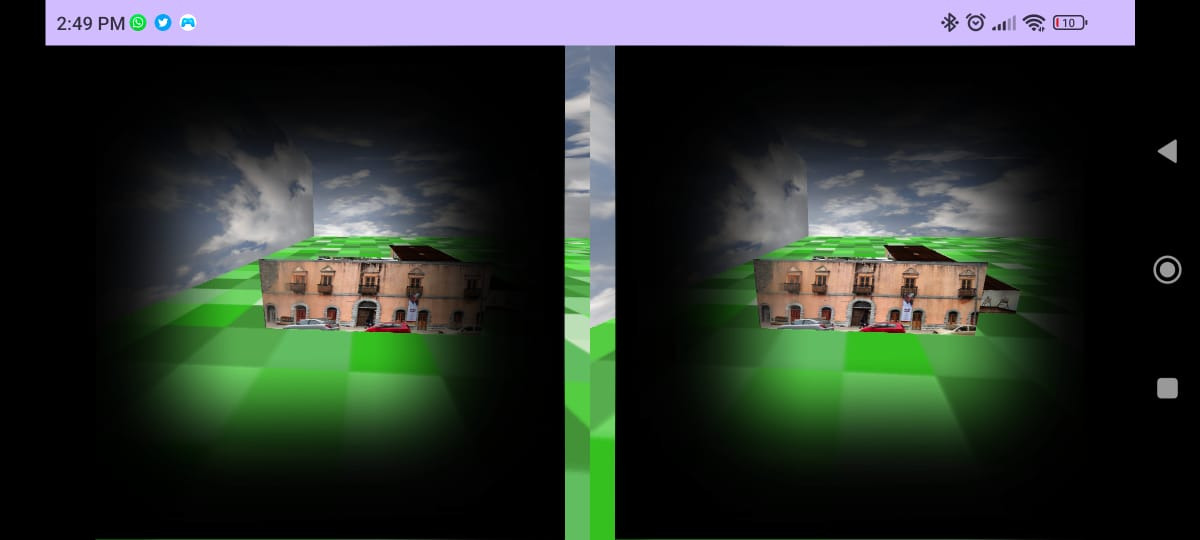
\includegraphics[width=0.40\linewidth]{2024_Pinacoteca_Virtual/PlanoGeneral.jpeg} &
 	%	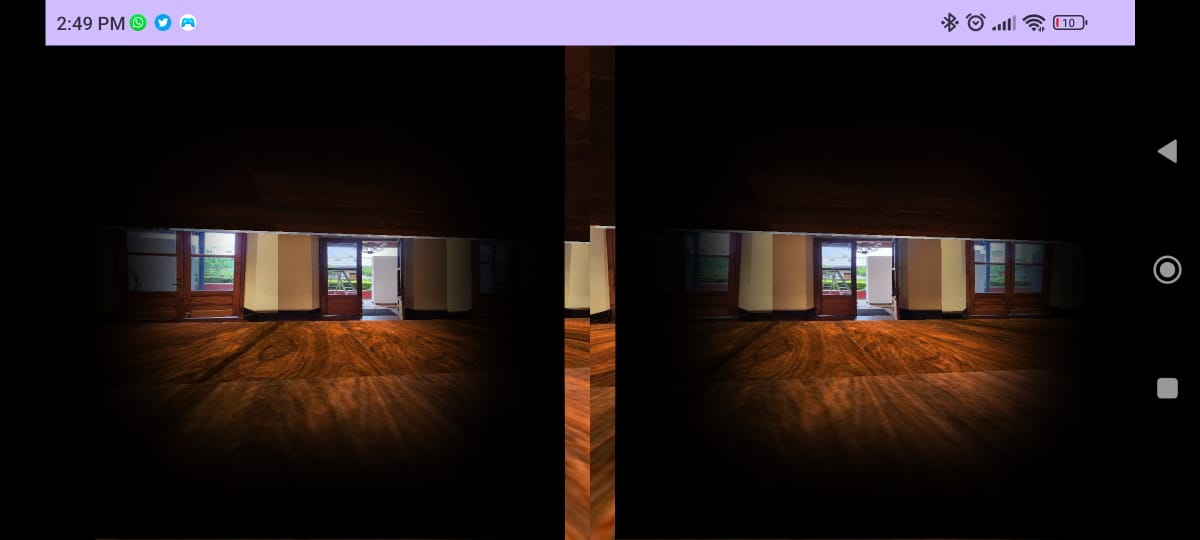
\includegraphics[width=0.40\linewidth]{2024_Pinacoteca_Virtual/Salida_SalonExhibiciones.jpeg} \\
%	\end{tabular}
%\end{center}


\end{columns}
\end{frame}


